% !TEX program = xelatex
\documentclass[10pt,letterpaper,twocolumn]{article}

\usepackage[top=0.75in, bottom=0.75in, left=0.75in, right=0.75in]{geometry}
\usepackage{fontspec}
\usepackage{unicode-math}
\setmainfont{Latin Modern Roman}[
  Extension=.otf,
  UprightFont=lmroman10-regular,
  BoldFont=lmroman10-bold,
  ItalicFont=lmroman10-italic,
  BoldItalicFont=lmroman10-bolditalic,
]
\setsansfont{Latin Modern Sans}[
  Extension=.otf,
  UprightFont=lmsans10-regular,
  BoldFont=lmsans10-bold,
  ItalicFont=lmsans10-oblique,
  BoldItalicFont=lmsans10-boldoblique,
]
\newfontfamily\acbold{ywft-processing-bold}[Path=../../system/public/type/webfonts/,Extension=.ttf]
\setmonofont{Latin Modern Mono}[
  Extension=.otf,
  UprightFont=lmmono10-regular,
  ItalicFont=lmmono10-italic,
  Scale=0.85,
]

\usepackage{xcolor}
\usepackage{titlesec}
\usepackage{enumitem}
\usepackage{booktabs}
\usepackage{tabularx}
\usepackage{fancyhdr}
\usepackage{hyperref}
\usepackage{xurl}
\usepackage{graphicx}
\graphicspath{{figures/}{../arxiv-ac/figures/}}
\usepackage{ragged2e}
\usepackage{microtype}
\usepackage{natbib}
\usepackage{tikz}
\usetikzlibrary{positioning,arrows.meta}

\definecolor{acpink}{RGB}{180,72,135}
\definecolor{acpurple}{RGB}{120,80,180}
\definecolor{acdark}{RGB}{64,56,74}
\definecolor{acgray}{RGB}{119,119,119}

\hypersetup{colorlinks=true,linkcolor=acpurple,urlcolor=acpurple,citecolor=acpurple,
  pdftitle={Paying for Strangers},
  pdfauthor={Jeffrey Scudder}}

\titleformat{\section}{\normalfont\bfseries\normalsize\uppercase}{\thesection.}{0.5em}{}
\titlespacing{\section}{0pt}{1.2em}{0.3em}
\titleformat{\subsection}{\normalfont\bfseries\small}{\thesubsection}{0.5em}{}
\titlespacing{\subsection}{0pt}{0.8em}{0.2em}

\newcommand{\acdot}{{\color{acpink}.}}
\newcommand{\ac}{Aesthetic{\acdot}Computer}

\pagestyle{fancy}\fancyhf{}
\renewcommand{\headrulewidth}{0pt}
\fancyhead[C]{\footnotesize\color{acpink}\textit{Field report --- \ac{} papers}}
\fancyfoot[C]{\footnotesize\thepage}

\newcommand{\code}[1]{\texttt{#1}}

\setlist[itemize]{nosep, leftmargin=1.2em, itemsep=0.1em}
\setlist[enumerate]{nosep, leftmargin=1.4em, itemsep=0.1em}
\setlength{\columnsep}{1.8em}
\setlength{\parindent}{1em}
\setlength{\parskip}{0.3em}

\tolerance=800
\emergencystretch=1em
\hyphenpenalty=50

\begin{document}

\twocolumn[{%
\begin{center}

\includegraphics[height=4em]{pals}\par\vspace{0.5em}
{\acbold\fontsize{21pt}{25pt}\selectfont\color{acdark} Paying for Strangers}\par
\vspace{0.45em}
{\normalfont\itshape\fontsize{11pt}{13pt}\selectfont\color{acpink} An unmetered inference endpoint, the handle that closed it, and what a day of it costs}\par
\vspace{0.3em}
{\normalfont\fontsize{9pt}{11pt}\selectfont\color{acgray} The payment rail was never the problem. Knowing who was asking was.}\par
\vspace{0.6em}
{\normalsize\href{https://prompt.ac/@jeffrey}{@jeffrey}}\par
{\small\color{acgray} \ac{} --- September 11, 2026}\par
{\small\color{acgray} ORCID: \href{https://orcid.org/0009-0007-4460-4913}{0009-0007-4460-4913}}\par
\vspace{0.3em}
{\small\color{acpurple} \url{https://aesthetic.computer}}\par
\vspace{0.6em}
\rule{\textwidth}{1.5pt}
\vspace{0.5em}
\end{center}

\begin{quote}
\small\noindent\textbf{Abstract.}
A companion report asked whether an art archive could sell itself to language-model
agents and answered, after building the turnstile, mostly no~\citep{scudder2026x402}.
Its strategy table left one option scored \emph{untested}: sell to handles rather
than to crawlers. This report takes up that option and finds that \ac{} had been
running the product already, for free, without noticing. \code{/api/ask} proxies
Anthropic and OpenAI on \ac{}'s own keys and backs four shipping features; its
entire authorization was a three-entry CORS origin allowlist, which is a browser
convention and not a check. The model was selected by a caller-supplied
\code{hint} field, so there was no ceiling on what a stranger could spend per
request, only on how many tokens came back. A sibling endpoint, \code{/run},
accepted unauthenticated writes to any live code channel, making the channel name
itself the credential. Both were closed in a day. Authorization now resolves an
\code{@handle} through the existing identity path; anonymous callers are clamped
to the cheapest model and 512 tokens rather than refused, because a free tier
that becomes an outage is a worse product than no free tier; and a handle
receives a daily token budget that degrades to the anonymous tier on exhaustion
rather than closing the door. We report production measurements from the
deployed system, and settle by experiment the question a prior cost analysis
could only pose: OpenRouter's per-key dollar limit is a hard server-side stop,
returning HTTP 403, and it fires \emph{early} --- the refusal arrived while the
readable counter still showed 39.6\% of the cap remaining, because that counter
is eventually consistent. For a cap whose purpose is bounding a bill, erring
early is the correct direction. We close with what the episode suggests about
failures that are invisible because nothing is broken.
\end{quote}
\vspace{0.5em}
}]

\section{Introduction}

A recurring question in this practice is where cultural value, once accumulated,
can be captured. A companion report put that question to language-model agents:
the \textsc{Whistlegraph} archive was fitted with an x402 paywall, priced, and
advertised to crawlers~\citep{scudder2026x402}. The answer was a negative result.
Two of the three priced endpoints computed their answers from files the same
site published for free, so a rational agent never paid; and across retained
logs, no agent ever asked. That report concluded that the binding constraints on
machine commerce are substitutability and discovery, not payment infrastructure,
and scored six strategies against those constraints. One, \emph{agent handles},
passed non-substitutability and was marked \emph{untested}.

This report tests the adjacent case. The buyer is not a crawler but a person
holding an \code{@handle}, and the good is not derived data but inference. The
finding is that the experiment had already been running. \ac{} has been buying
language-model inference for anonymous strangers since the feature shipped,
through an endpoint nobody thought of as a product because it had never been
priced, metered, or gated.

Section~\ref{sec:context} describes the surface. Section~\ref{sec:defect} is the
audit. Section~\ref{sec:system} describes what replaced it, and
Section~\ref{sec:impl} how. Section~\ref{sec:evidence} reports measurements from
production, including an experiment that settles a question a prior cost analysis
could only pose. Section~\ref{sec:limits} states what this does not establish.

\section{Context}
\label{sec:context}

\ac{} is a mobile-first runtime and social network for creative computing, in
which programs are addressable \emph{pieces}~\citep{scudder2026pieces} and
identity is an \code{@handle} resolved through Auth0 against a MongoDB
collection. Four shipping features call language models: \code{make} and
\code{paint}, which generate pieces from a described intent; \code{translate};
and the prompt system itself. All four route through one client module,
\code{lib/ask.mjs}, to one backend function, \code{/api/ask}.

That function is 616 lines and proxies two vendors --- \code{api.anthropic.com}
and \code{api.openai.com} --- using API keys held in \ac{}'s production
environment. It is, in every respect except that nobody called it one, a hosted
AI service with a free and unlimited tier.

\section{The audit}
\label{sec:defect}

Three defects were found, in ascending order of consequence.

\subsection{An origin header is not a credential}

The whole of \code{/api/ask}'s authorization was:

\begin{quote}
\small\code{if (!dev \&\& !allowedOrigins.includes(origin))}\\
\small\code{\ \ return \{ statusCode: 403 \};}
\end{quote}

\noindent against a three-entry allowlist. The \code{Origin} header is a browser
convention: browsers set it honestly and refuse to let page scripts forge it,
which is what makes CORS useful \emph{to browsers}~\citep{fetchcors}. Nothing else is obliged to
participate. Any client that is not a browser --- \code{curl}, a script, a
crawler --- simply sends the string. The control was doing real work against the
threat it was designed for, cross-origin reads by a page, and no work at all
against the one that mattered here, which is cost.

\subsection{The caller chose the model}

More consequential, and less visible. The model was parsed out of a
caller-supplied \code{hint} field. A request could name any model the proxy
would forward, including the most expensive available. The only ceiling in the
code was \code{max\_tokens}, which bounds the response but not the price of
producing it. An anonymous caller could therefore select \ac{}'s cost per
request, and the difference between the cheapest and dearest model on offer is
roughly a factor of thirty.

\subsection{A channel name as a credential}

A sibling endpoint, \code{/run}, accepted \code{\{piece, source, codeChannel\}}
and published the source to a Redis channel, from which any subscribed browser
would execute it. It required no authentication and set
\code{Access-Control-Allow-Origin: *}. Its protection was that channel names
were unguessable: eight base64url characters, minted client-side, and documented
in the source as ``a shared secret\ldots{} make it unguessable.''

This is a defensible design until the moment something needs to \emph{publish}
the channel name --- which is exactly what a live-coding session wants to do, so
that a phone can scan a code and watch the piece being written. Secrecy and
addressability are incompatible requirements on the same string.

\section{System}
\label{sec:system}

The replacement rests on one move: ownership migrates from the secrecy of a name
to the possession of a token.

\subsection{Ownership is a check, not a secret}

A code channel is now written \code{<handle>/<slug>}. A push to it is accepted
only when the request carries an access token resolving to that handle, verified
through the same \code{authorize()} path other authenticated endpoints already
use. The name no longer needs to hide, so it can be published --- and since it
can be published, it can be the piece's public address as well.

Table~\ref{tab:run} gives the resulting behaviour, measured against production.

\begin{table}[t]
\centering
\footnotesize
\begin{tabularx}{\columnwidth}{@{}Xl@{}}
\toprule
\textbf{Request to \code{/run}} & \textbf{Response} \\
\midrule
No credentials & 410 Gone \\
Invalid token & 401 \\
\code{@jeffrey} $\rightarrow$ \code{jeffrey/\dots} & 200 \\
\code{@jeffrey} $\rightarrow$ \code{someoneelse/\dots} & 403 \\
\bottomrule
\end{tabularx}
\caption{Observed responses from the deployed endpoint. Anonymous requests
answer 410 rather than 401 because the condition is expected to be
permanent~\citep{rfc9110}: there is no way to retry the request as written.}
\label{tab:run}
\end{table}

\begin{figure}[t]
\centering
\footnotesize
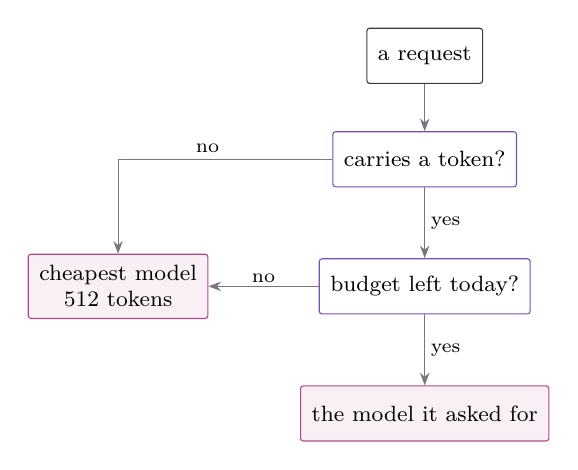
\begin{tikzpicture}[
  node distance=6mm,
  box/.style={draw=acdark, rounded corners=1pt, align=center, inner sep=4pt,
              minimum height=7mm, font=\footnotesize},
  ask/.style={box, draw=acpurple},
  tier/.style={box, fill=acpink!8, draw=acpink},
  line/.style={-{Stealth[length=1.6mm]}, draw=acdark!70},
]
\node[box] (req) {a request};
\node[ask, below=of req] (tok) {carries a token?};
\node[ask, below=9mm of tok] (bud) {budget left today?};
\node[tier, below=9mm of bud] (full) {the model it asked for};
\node[tier, left=14mm of bud] (cheap) {cheapest model\\512 tokens};

\draw[line] (req) -- (tok);
\draw[line] (tok) -- node[right, font=\scriptsize, inner sep=2pt] {yes} (bud);
\draw[line] (bud) -- node[right, font=\scriptsize, inner sep=2pt] {yes} (full);
\draw[line] (tok.west) -| node[above left, font=\scriptsize, inner sep=2pt, pos=0.25] {no} (cheap.north);
\draw[line] (bud.west) -- node[above, font=\scriptsize, inner sep=1pt] {no} (cheap.east);
\end{tikzpicture}
\caption{How a request to \code{/api/ask} is priced. The two ways of not
qualifying --- no identity, and an identity that has spent its day --- arrive at
the same place, and that convergence is the design rather than an economy of
implementation. Neither is a refusal: the feature answers in both cases, more
cheaply. A budget that becomes an outage would be worse than no budget.}
\label{fig:tier}
\end{figure}

\subsection{A tier, not a wall}

For \code{/api/ask} the design question is different. Refusing anonymous callers
would be cheapest and would also break the front page for anyone who has never
logged in, which is most first visitors to a creative tool. So anonymous traffic
is not refused; it is \emph{clamped}, to the cheapest model and 512 tokens,
regardless of what \code{hint} requests (Figure~\ref{fig:tier}). The demo still demos. It costs roughly a
tenth of what it did.

A request carrying a valid token reaches the model it asked for. That is the
first thing a handle buys, and it is a concrete answer to the strategy the prior
report left untested: the good sold is not data, which an agent can recompute,
but access priced by identity.

\subsection{A day, not a balance}

Each handle receives a token budget per UTC day. The bucket is a day rather than
a month because a monthly pool can be drained in an afternoon, leaving the tool
dead for three weeks --- the worst possible shape for someone who opened an
editor to make something. A day resets: the bad outcome is ``come back
tomorrow,'' and exposure is bounded at roughly thirty times a day's spend.

Exhaustion degrades rather than refuses. A handle over budget is served exactly
as a visitor is. Every failure in the system leans the same way deliberately: a
budget lookup that errors reads as \emph{unspent}, and the usage write is
fire-and-forget after the response is already delivered. Over-serving through a
database blip is recoverable; losing a user's reply to an accounting race is not.

\section{Implementation}
\label{sec:impl}

Three notes on implementation that cost time and may cost someone else time.

\textbf{Module systems.} The gate was first added to \code{/api/ask} as a static
ESM \code{import} at the top of a file whose first line is
\code{require("@netlify/functions")}. Mixing the two does not raise: the module
fails to load, and the host answers \code{404 Function not found}. Four shipping
features went silent without an error anywhere. A dynamic \code{import()} inside
the handler is legal in CommonJS and resolves the same module.

\textbf{Client identity.} \code{Conversation}, the client-side wrapper, is
constructed in five places with only a store and a slug, and had no route to a
token. Rather than thread one through every caller, a module-level provider is
installed once at boot and resolves the token at call time, so signing in or out
is reflected on the next request with no cache to invalidate. A missing token is
not an error; it is the anonymous path.

\textbf{A file that could not be searched.} \code{disk.mjs}, the 17,000-line
client core, contained a literal NUL byte used as a cache-key separator. This is
legal JavaScript. It also causes \code{file} to report the source as
\code{data} and every \code{grep} over it to match nothing --- silently, with no
error and no warning. Four searches for the channel-subscription code returned
empty before the cause was found, and the provisional conclusion that the
feature had been deleted was wrong. The byte is now written \code{\textbackslash
0}, which is the same string.

\section{Evidence}
\label{sec:evidence}

All measurements are from the deployed production system on 11 September 2026.

\subsection{Tier selection}

The endpoint logs its decision. Anonymous requests naming an expensive model are
rewritten; authenticated requests are not, and carry the remaining budget:

\begin{quote}
\small\code{Anonymous --- gpt-4o $\rightarrow$ gpt-4o-mini}\\
\small\code{@jeffrey --- gpt-4o $\cdot$ 25000/25000 left}\\
\small\code{@jeffrey --- gpt-4o $\cdot$ 24988/25000 left}\\
\small\code{@jeffrey --- gpt-4o $\cdot$ 24975/25000 left}
\end{quote}

\noindent The decrement is real usage reported by the provider, not an estimate.
Both vendor paths already parsed token counts in order to draw a progress bar in
the server log; the accounting reuses those numbers, so neither path had to learn
anything new.

\subsection{Addressing costs a QR version}

Because the channel name became publishable, the scanned address could become
the piece's published URL rather than a throwaway route. The cost is measurable.
At error-correction level L, a version-2 symbol holds 32 bytes in byte
mode~\citep{qrspec}.
\code{https://prompt.ac/\textasciitilde l\_mUYjNq} is 27 and fits;
\code{https://prompt.ac/@jeffrey/murafi} is 33 and does not, promoting the symbol
from 25$\times$25 modules to 29$\times$29. One byte over. The gain is an address
that outlives the session.

\subsection{The per-key limit is a hard stop}

A prior cost analysis proposed minting a dollar-capped OpenRouter key per handle,
but could not establish whether \code{limit} is enforced or merely recorded ---
the documentation exposes \code{limit\_remaining} and never states what happens
to a request that would exceed it~\citep{openrouterkeys}. The distinction decides whether a runaway user
is stopped or merely observed.

We minted a key capped at \$0.0005 and spent past it. Table~\ref{tab:probe} gives
the run.

\begin{table}[t]
\centering
\footnotesize
\begin{tabularx}{\columnwidth}{@{}clXr@{}}
\toprule
\textbf{Call} & \textbf{HTTP} & \textbf{Reported usage} & \textbf{Remaining} \\
\midrule
1 & 200 & \$0         & \$0.000500 \\
2 & 200 & \$0         & \$0.000500 \\
3 & 200 & \$0.0003021 & \$0.000198 \\
4 & 200 & \$0.0003021 & \$0.000198 \\
5 & \textbf{403} & \$0.0003021 & \$0.000198 \\
\bottomrule
\end{tabularx}
\caption{Spending past a \$0.0005 per-key cap. The refusal
(\emph{``Key limit exceeded (total limit)''}) arrives while the readable counter
still reports 39.6\% of the cap available, because that counter is eventually
consistent --- note it is unchanged across calls 3--5.}
\label{tab:probe}
\end{table}

Two findings follow. The limit is a genuine server-side stop, returning HTTP 403.
And enforcement runs \emph{ahead} of the number a client can read: the refusal
fired while \code{limit\_remaining} still showed \$0.000198, because the usage
counter updates in jumps every three or four calls. \code{limit\_remaining} is
therefore an observation and never a prediction. The discrepancy leans toward
refusing early rather than overspending, which for a cap whose purpose is
bounding a bill is the correct direction to be wrong in.

Two further claims were verified in passing. OpenRouter's endpoint compatible with the Anthropic
Messages API~\citep{anthropicmessages} returns a correctly shaped response including a
\code{cost} field in dollars per call --- which would permit metering in money
rather than in estimated tokens, eliminating drift between a token budget and an
actual bill as prices change. And the vendor CLI that the editor's bridge already
drives connects to OpenRouter given three environment variables and no code
change, so an alternative backend is a configuration entry rather than a new
protocol. The entire investigation cost \$0.086.

\section{Ethics, privacy, and limitations}
\label{sec:limits}

\textbf{What this does not establish.} We report the behaviour of one deployment
over one day. The daily budget figure was chosen before usage data existed to
choose it from, and is deliberately an environment variable rather than a
constant; it should be set from the collected data and is not yet. We did not
measure whether the anonymous tier's cheaper model degrades the four features
enough to matter to a first-time visitor, which is the central product risk of
the clamp and wants a user study rather than a log line. Our own registered-handle
count could not be verified for this report: the public endpoint returns a capped
page of 100, and a figure of 2,814 obtained from another source is repeated here
only as unverified.

\textbf{Privacy.} The gate reads an identity in order to price a request. It
stores a token count and a model name per handle per day, and no prompt content.
This is a real expansion of what is recorded about a user --- previously nothing
was --- and it is the minimum that metering requires. Prompts continue to leave
the machine to two vendors, which was true before this work and is disclosed in
the interface.

\textbf{Disclosure.} This report describes defects in a system the author
operates, both now closed, and names no third party's vulnerability.

\section{Conclusion}
\label{sec:conclusion}

The prior report found that a turnstile for machines earns nothing when the good
behind it is substitutable and undiscoverable. This one finds the complement: a
turnstile that was never built, on a good that is neither --- inference cannot be
recomputed by the buyer, and the buyer was already standing at the door.

What made the omission durable is worth naming, because it is not carelessness.
Every individual piece was reasonable. An origin allowlist is a real control
against a real threat. A caller-chosen model is a feature. An unguessable channel
is a legitimate capability pattern. Nothing failed, no error was logged, no
alarm existed to fire, and the endpoint answered every request correctly and
promptly for as long as it existed. The system was not broken; it was working
exactly as built, and what it was built to do included something nobody had
decided.

A related failure sat one directory away during this work: the documentation
promised that pushing a paper rebuilds its PDF within a minute, and that had
not happened since May, because an emergency pause added by hand during an
incident outlived its cause by four months. It was invisible for the same
reason. The promise was in a document, the contradiction was a \code{false} in a
JSON response nobody read, and the papers were never stale --- because they were
being built by hand, which is precisely what kept the automation's absence from
being noticed.

Both are the same class of defect: a gap between what a system is understood to
do and what it does, held open by the absence of anything that would announce
the difference. The gate is the cheap part. Knowing who is asking, and having
somewhere that says so out loud, is the whole of it.

\bibliographystyle{plainnat}
\bibliography{references}

\end{document}
